\part[Электродинамика и распределение радиоволн]{
Электродинамика и распределение радиоволн \\
{\Large Симушин Алексей Александрович}
}

\part{2025-02-07. Поля и операции вектороного поля}

\begin{itemize}
	\item Поток вектора $F$ через поверхность $S$: \[ \Phi = \int_S \vec{F dS}. \]
	      Определение поверхности определяет нормаль. В потоке может учавствовать
	      только нормальная составляющая, тангенциальная ``скользит'' по
	      поверхности.
	\item $dS = V_n dS$ отсюда $F dS = F_n dS$;
	      \begin{itemize}
		      \item $\Phi > 0$ --- исток;
		      \item $\Phi < 0$ --- сток;
		      \item $\Phi = 0$ --- не исток, не сток.
	      \end{itemize}
\end{itemize}

\begin{figure}[htbp]
	\centering
	\begin{subfigure}[h]{0.25\textwidth}
		\centering
		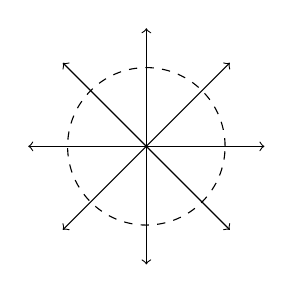
\begin{tikzpicture}[scale=0.5]
			\draw[dashed] (0, 0) circle (2);
			\foreach \x in {0, 45, ..., 315} {
					\draw[->] (0, 0) -- (\x:3);
				}
		\end{tikzpicture}
		\caption{Исток}
	\end{subfigure}
	\begin{subfigure}[h]{0.25\textwidth}
		\centering
		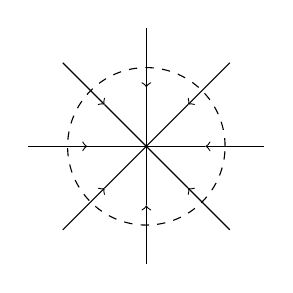
\begin{tikzpicture}[scale=0.5]
			\draw[dashed] (0, 0) circle (2);
			\foreach \x in {0, 45, ..., 315} {
					\draw[->] (\x:3) -- (\x:1.5);
					\draw (\x:1.5) -- (\x:0);
				}
		\end{tikzpicture}
		\caption{Сток}
	\end{subfigure}
\end{figure}

\subsubsection{Дивергенция}

Рассмотрим поток через малый параллелипипед: \[ d\Phi = \oint_S \vec{F} d\vec{S}
	= \oint F_n dS, \] $F_n$ --- нормальная, составляющая к поверхности
параллелипипеда, постоянна.

Поток через правую грань: $F_n^\text{пр} (x+\Delta x, y_\text{ср}, z_\text{ср})
	dS = F_x^\text{пр} (x+\Delta x, y_\text{ср}, z_\text{ср}) dydz$.

Разность $F_n^\text{пр} - F_n^\text{лев}$ есть приращение.

Поток вектора через любую замкнутую поверхность
\[ \Phi = \sum_{}^{} d\Phi = \sum \vec{F} d\vec{V}. \]
Поскольку изначально тот же поток $\Phi = \int_S \vec{F} d\vec{S}$.

\[
	\boxed{\oint_S = \vec{F} d\vec{S} = \int_V \dive \vec{F} dV}
\]
Теорема Остроградского--Гауса\index{Теорема~Остроградского--Гауса}.

\subsubsection{Ротор}

Рассмотрим интеграл вектора $F$ по малому контуру $ABCD$ \[ dC = \oint_l \vec{F}
	d\vec{l} = \oint_l F_l dl. \]
Если контур замкнут, то интеграл называется циркуляцией\index{Циркуляция}.

\begin{figure}[!htbp]
	\centering
	\begin{tikzpicture}[tdplot_main_coords]
		\coordsystemd{0}{0}{0}{3}{3}{3}

		\draw (0, 0, 0) circle (2);
		\draw[dashed] (-2, -2, 0) node[above] {$A$} -- (2, -2, 0)
		node[left] {$B$} -- (2, 2, 0) node[below] {$C$} -- (-2, 2, 0)
		node[right] {$D$} -- cycle;
	\end{tikzpicture}
	\caption{<caption>}
\end{figure}

\[
	dC = \oint_l F_L dl = F_x' \Delta x + F_y' \Delta y + F_z' \Delta z - F_x''
	\Delta x - F_y'' \Delta y
	.\]

Таким образом, для любого малого прямоугольника
\begin{align*}
	dC           & = \oint_l F_L dl = \rot(F) dS \\
	\rot \vec{F} & =
	\begin{vmatrix}
		\vec{i}                      & \vec{j} & \vec{k} \\
		\sfrac{\partial}{\partial x} &
		\sfrac{\partial}{\partial x} &
		\sfrac{\partial}{\partial x}                     \\
		F_x                          & F_y     & F_z
	\end{vmatrix}
	.
\end{align*}

Для любого контура произвольных размеров
\[
	C = \sum_{}^{} dC = \sum_{}^{} \oint F_L dl = \sum_{}^{} \rot_n \vec{F}
	d\vec{S} = \int \rot_n \vec{F} d\vec{S}
	.\]

Но изначально для того же контура $C = \oint_L \vec{F} d\vec{l}$ поэтому
\[
	C = \oint_L \vec{F} d\vec{l} = \int_S \rot_n \vec{F} d\vec{S}
	,\]
где $S$ --- площадь, ограниченная контуром $L$.

Ротор\index{Ротор} (вихрь векторного поля $F$) --- векторная характеристика
``вращательной составляющей'' векторного поля $F$.

\begin{itemize}
	\item Для любого потенциального поля $F = \nabla \varphi$ имеем $\rot F=0$, то
	      есть $\rot(\nabla \varphi) = 0$;
	\item Для любого соленоидального поля $F = \rot V$ имеем $\dive F = 0$;
	\item Если в векторном анализе известны и ротор и дивергенция, то поле
	      считается определённым;
\end{itemize}

\section{Электромагнитное поле}

Электромагнитные явления делят на две группы: электрические и магнитные.
Соответственно, поле делят на электростатические и манитные разновидности.
Электростатическое поле:
\[ F_k(r) = qE(r) \qquad E\left[\unit{\volt\per\meter}\right] \]
Электрическое поле в вакууме:
\[ D = \varepsilon_0 E \qquad D\left[\unit{\coulomb\per\square\meter}\right], \]
$\varepsilon_0 = \qty{8.845e-12}{\farad\per\meter} \approx
	\frac{1}{36\pi \cdot 10^9}$.

Индукция --- это параметр, который определяется только \dots

Магнитное поле в магнетиках:
\[ F_L = q[V, B] \qquad B[\unit{\tesla}] \]
Магнитное поле в вакууме:
\[ B = \mu_0 H \qquad H\left[\unit{\ampere\per\meter}\right], \]
где $\mu_0 = 4\pi \cdot 10^{-7} \unit{\henry\per\meter}$ --- магнитная
постоянная.

Колебания параметров $E, D, B, H$ порождает электромагнитные волны.

\subsubsection{Ток проводимости}

\begin{definition}[Ток проводимости]
	Упорядоченное движение заряженных частиц. Плотность тока --- показатель,
	представляющий ток, как векторное поле.

	$j\left[\unit{\ampere\per\meter}\right]$, $j_\text{пр} = nq \upsilon$
	\begin{equation*}
		J = \int_S j dS
	\end{equation*}
\end{definition}

\paragraph{Дифференциальный закон Ома}
\[
	j_\text{пр} = \sigma E
	,\]
где $\sigma [\unit{\siemens\per\meter}]$ --- удельная проводимость.

\subsubsection{Закон сохранения заряда}
